% !TeX spellcheck = en_US

\chapter{Implementation}
\label{chap:implementation}

\section{Technology Stack}
The implementation of the chatbot system leverages a diverse set of technologies, each chosen for its specific capabilities and compatibility with the existing Bosch Smart Home ecosystem. Figure \ref{fig:techstack} illustrates the technology stack overlaid on the base architecture.

Android Studio serves as the primary integrated development environment, facilitating the extension of the existing Bosch Smart Home Android application. The client-side development utilizes Java programming language in conjunction with Android 14 SDK, ensuring compatibility with the latest Android features and optimizations.

To enhance the user interface and manage the chat functionality efficiently, the implementation incorporates modern Android components. RecyclerView is employed for rendering the message exchange between the user and the chatbot, providing smooth scrolling and efficient memory usage. Concurrency tools, specifically ExecutorService and CompletableFuture, are utilized to handle API calls in the background, ensuring a responsive user interface while managing asynchronous operations.

On the server side, Ollama v0.1.47 is deployed for hosting, customizing, and invoking the language model. The Ollama API facilitates seamless interaction between the client application and the server-hosted language model.

\gls{json} serves as the primary data exchange format between the server and client components. This lightweight and human-readable format is used both for constructing API calls to the Ollama API and for transmitting the language model's responses back to the client.
\begin{figure}[h]
    \centering
    \captionsetup{justification=centering}
    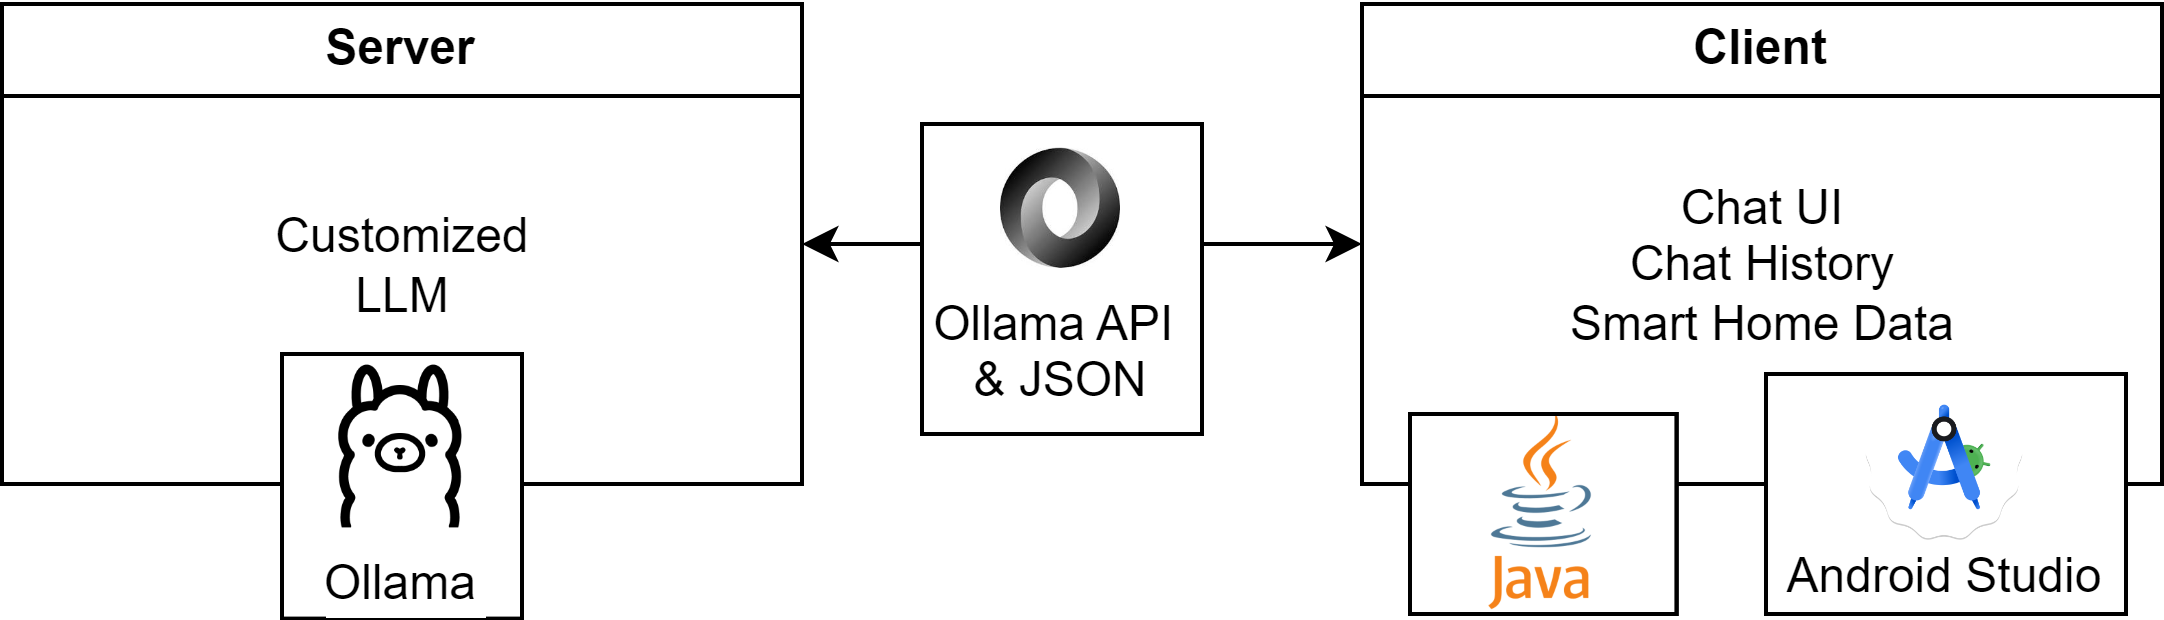
\includegraphics[width=0.9\textwidth]{graphics/techstack.png}
    \caption{Technology stack visualized on base architecture}
    \label{fig:techstack}
\end{figure}

\section{Server}
The initial plan was to use the bwCloud\footnote{\url{https://www.bw-cloud.org/}}, a currently free service that can be used of students and researchers of different institutions accross Baden-Würrtemberg, Germany.
It was easy to get the needed ressources for this project which where eigth VCPUs, 16GB RAM and also enough memory for the size of the \glspl{llm} that were planned to use.
When trying out to run models directly on the server the response times were okay for models up to approximately 10 Billion perameters although the used server has no GPU.
However, when testing customized models through HTTP Requests the response times were much higher than expected.
Especially the first response often took over one minute with preceeding requests taking minimum 30 seconds depending on the length of the generated respone.
The first request usually takes longer when the model used is not allready loaded into the RAM.

Because of the occuring difficulties and with wanting to use as low budget as possible we decided to use an existing private Computer with more Ressources and used IPv6 Host Exposure for a specific port on which the Ollama API was running.
The computer had an NVIDIA GeForce 980 ti graphics card with 6GB VRAM and 32GB RAM with 3600MHz.
Even longer model responses usually only took a few seconds to receive.

\section{Model Customization}
This section is all about the language models themselves. It covers which model where selected and why, how the models where customized with so called "Modelfiles" and an engineered prompt.
\subsection{Model Selection}
The model selection was based on parameter count, popularity, ranking in the \gls{bfcl} and availability in the ollama models library.
The parameter count should be lower than 15 Billion since it wouldn't really run on the server setup described in the last section.
The model should be either under the most popular models filter on the Ollama library website \footnote{\url{https://ollama.com/library?sort=popular}}

"home-3b-v3",
"qwen2-7b-instruct",
"sqwen2-1.5b-instruct",
"mistral-7b-instruct",
"gemma-2b-instruct",
"gemma-instruct",
"zephyr",
"llama3",
"llama3-instruct"
"phi3"
%TODO add gorilla, fireflies, new gemini/gemma model?
\subsection{Modelfiles}
\subsection{Prompt Engineering}


\section{Data Management}

\section{User Interface}
\subsection{Chatbot in Action}
\section{Challenges and Solutions}
Several challenges and considerations were addressed during the design and development of the prototype:

\begin{itemize}
\item \textbf{Complexity of Automations}: Balancing simplicity and functionality in user-defined automations.
\item \textbf{Multilingual Support}: Providing accurate and contextually appropriate responses in both German and English.
\item \textbf{Historical Data}: ...
\item \textbf{Availability of System Logs}: ...
\item \textbf{Security Issue}: trusted domains
\end{itemize}
%\blinddocument
